\section{Route Designer Web Page}

For this sprint, a route designer web page was desired. Its functionality should include a map where users could create and modify routes, as well as a user login system to restrict access to a user's own routes.

\section{Graphical User Interface}

A simple user interface was needed. An initial mock-up can be seen in \autoref{fig:sprint1-web-ui}, which shows the desired layout of the route planner display. The general philosophy was to keep the layout consistent on all pages. As such, the title and the menu will be at the same position on all views, though the menu options will change depending on the permissions of the user, in this case whether the user is logged in or not.

\begin{figure}[ht]
 \caption{Web UI Mock up}
 \label{fig:sprint1-web-ui}
 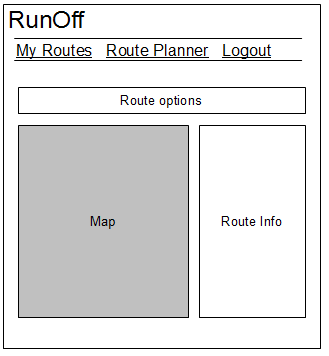
\includegraphics[scale=1]{img/webmockup1.png}
\end{figure}

Four views, which should constitute an \ac{MVP}, were planned for this sprint:
\begin{itemize}
 \item {Route Designer} (Only available when logged in)
 \item {Route Overview} (Only available when logged in)
 \item {User Registration}
 \item {User Log In}
\end{itemize}

The route overview should be a simple listing of the routes the current user has created, with a summary of the information available for that route, as well as a link to modify each route. The registration and log in views should be simple \ac{HTML} forms.
